
%%%%%%%%%%%%%%%%%%%%%%% file typeinst.tex %%%%%%%%%%%%%%%%%%%%%%%%%
%
% This is the LaTeX source for the instructions to authors using
% the LaTeX document class 'llncs.cls' for contributions to
% the Lecture Notes in Computer Sciences series.
% http://www.springer.com/lncs       Springer Heidelberg 2006/05/04
%
% It may be used as a template for your own input - copy it
% to a new file with a new name and use it as the basis
% for your article.
%
% NB: the document class 'llncs' has its own and detailed documentation, see
% ftp://ftp.springer.de/data/pubftp/pub/tex/latex/llncs/latex2e/llncsdoc.pdf
%
%%%%%%%%%%%%%%%%%%%%%%%%%%%%%%%%%%%%%%%%%%%%%%%%%%%%%%%%%%%%%%%%%%%


\documentclass[runningheads,a4paper]{llncs}

\usepackage{amssymb}
\usepackage{amsmath}
\setcounter{tocdepth}{3}

\usepackage{graphicx}
\graphicspath{{./pdf/}}
\DeclareGraphicsExtensions{.pdf}

\usepackage{subfigure}
\usepackage{url}
\usepackage{multirow,booktabs,makecell,color,colortbl}
 
\newcommand{\keywords}[1]{\par\addvspace\baselineskip
\noindent\keywordname\enspace\ignorespaces#1}

\begin{document}

\mainmatter  % start of an individual contribution

% first the title is needed
\title{Accelerating Multiple Sets Intersection with SIMD Instructions}
%XXX: An Insight into the Code-level Paralellism of Multiple Sets Intersection

% a short form should be given in case it is too long for the running head
\titlerunning{Accelerating Multiple Sets Intersection with SIMD Instructions}

% the name(s) of the author(s) follow(s) next
%
% NB: Chinese authors should write their first names(s) in front of
% their surnames. This ensures that the names appear correctly in
% the running heads and the author index.
%
\author{Xingshen Song \and Yuexiang Yang}
%
\authorrunning{Xingshen Song and Yuexiang Yang}
% (feature abused for this document to repeat the title also on left hand pages)

% the affiliations are given next; don't give your e-mail address
% unless you accept that it will be published
\institute{College of Computer,\\
National University of Defense Technology\\
Changsha, China\\
\email{\{songxingshen, yyx\}@nudt.edu.cn}}

% 
% NB: a more complex sample for affiliations and the mapping to the
% corresponding authors can be found in the file "llncs.dem"
% (search for the string "\mainmatter" where a contribution starts).
% "llncs.dem" accompanies the document class "llncs.cls".
%

\toctitle{Accelerating Multiple Sets Intersection with SIMD Instructions}
\tocauthor{Xingshen Song and Yuexiang Yang}
\maketitle


\begin{abstract}
Conjunctive Boolean query is one fundamental operation for document retrieval in many information systems and databases.
In its most basic and popular form, a conjunctive query can be seen as the intersection problem of multiple sets of sorted integers.
Various algorithms have been put up in terms of maximizing the query efficiency.
In recent years, researcher began to exploit the parallel advantage of single-instruction-multiple-data (SIMD) instructions to accelerate the intersection procedure and achieved substantial gains over previous scalar algorithms.
However, these works only focus on intersecting two sets at a time rather than the whole lot of them.
Missing from the literature is a thorough study that explores the combination of traditional multiple sets intersection algorithms and SIMD instructions.
In this article, we first revise all the 
%Inverted index is a key component for search engine to manage billions of documents and fast respond to users' queries. While substantial effort has been made to compromise space occupancy and decoding speed, what has been overlooked is the encoding speed when constructing the index. VSEncoding is a powerful encoder that works by optimally partitioning a list of integers into blocks which are efficiently compressed by using simple encoders, however, these partitions are found by using a dynamic programming approach which is obviously inefficient. In this paper, we introduce compression speed as one criterion to evaluate compression techniques, and thoroughly analyze performances of different partitioning strategies. A linear-time optimization is also proposed, to enhance VSEncoding with faster compression speed and more flexibility to partition an index. Experiments show that our method offers a far more better compression speed, while retaining an excellent space occupancy and decompression speed.
\keywords{Set Intersection, Algorithm Optimization, Vectorized Processing, Performance Evaluation}
\end{abstract}


\section{Introduction}\label{sec:introduction}
Conjunctive Boolean query is a common operation in information retrieval, it provides infrastructure for many complicated queries like ranked query or fuzzy query.
Namely, conjunctive query is to extract common elements from target sets and is widely used for document retrieval or text searching.
In nowadays information systems, inverted index is a prevailing data structure that has been generally applied for storage and query processing \cite{culpepper2010efficient,zobel2006inverted}.
An Inverted index can be seen as a big table mapping each unique \textit{term} to a \textit{posting list} which contains all the occurring document identifiers.
Thus, conjunctive query \textit{q} is computing the intersection of $ |q| $ sets of sorted integers.
The inflating size of web data and users has brought intense pressure on the query processing speed of information systems, in order to alleviate this dichotomy, a lot of research has been done to improve the efficiency of set intersection.
The earliest work can be dating back to decades ago \cite{Hwang1971Optimal,Hwang1972A}.

It is well known that there hardly exists a snake-oil method that suits for every scenario of intersections, the number of participating sets, the length ratio among them and the \textit{selectivity} (the ratio of intersection size to the smallest set size) will have tremendous impact on the efficiency of intersection algorithms.
Besides, different algorithms have distinctive features and advantages.
The straightforward method is called \texttt{Zipper} \cite{Sanders2007Intersection}, which works in a merge-wise fashion.
Given two sets whose length are $ m $ and $ n $ respectively (we always assume $ m<n $), \texttt{Zipper} needs time $ O( m + n ) $ and works well if both lists are of similar length.
Another algorithm that is designed for intersecting two sets is called \texttt{BaezaYates} \cite{Baeza2010Fast,Baezayates2004A,Baezayates2005Experimental}.
It recursively bisects the longer subset using the median element of the smaller subset until any subset becomes empty, achieving $ O(m\log (n/m)) $ time complexity.
The whole procedure works like the classic Quick Sort.

When it comes to the intersection of multiple sets, the comparison model begins to diverge, the first is called \texttt{small\_vs\_small}, each time the smallest sets is picked out, and in turn intersect it against each of the others, in increasing order of size.
\texttt{Zipper} and \texttt{BaezaYates} can be seen as two special cases where the number of sets are two.
Another model is called Holistic Intersection \cite{culpepper2010efficient}, namely to process all sets simultaneously and determine the elements in their intersection in an interleaved manner \cite{Culpepper2007Compact}.
The way these algorithms choose the searching element (called \textit{eliminator}) and how they search for it derives out a lot of varieties in the practical application.
Examples are \texttt{set\_vs\_set}, \texttt{Adaptive} \cite{Barbay2006Faster,Demaine2000Adaptive,Demaine2001Experiments}, \texttt{Sequential} \cite{Barbay2002Adaptive,Barbay2003Optimality} and \texttt{MaxSuccessor} \cite{Culpepper2007Compact}.

There also exist other approaches that try to solve the intersection problem from another perspectives.
Some build auxiliary data structures like treaps \cite{Blelloch1998Fast,chen2016efficient}, wavelet trees \cite{navarro2010dual}, skipping lists \cite{Culpepper2007Compact,Moffat1996Self} and hash tables \cite{Arroyuelo2010Compressed,Sanders2007Intersection} to facilitate random access and avoid redundant comprisons.
Some utilize modern hardware like GPU \cite{Ao2011Efficient,Wu2009A,Wu2010Efficient} or multi-core CPU \cite{Tatikonda2009On,tsirogiannis2009improving} to enable parallel processing.
However, these methods either need additional preprocessing or have special requirements on the target sets \cite{Inoue2014Faster}.

Recently, researchers begin to use SIMD instructions to boost the intersection performance \cite{Inoue2014Faster,Schlegel2010Fast,lemire2016simd}.
By exploiting the code-level parallelism and larger registers, SIMD-based methods are able to compare 4 or more elements at a time, and have shown substantial improvements over the scalar instructions.
% XXX:simply desccibe these simd-based method? for example???
Unfortunately, these methods only focus on the intersection of two sets, the way they execute the computation is more like vectorized \texttt{Zipper}, which restricts their scope of application to the sets with similar length and large selectivity.
Missing from the literature is a thorough empirical study that deploys SIMD instructions into multiple sets intersection algorithms and extensively measures their computation performances.

% 简述本文的工作,要不要按照点以item的形式列出来?
In this paper, we 
%使用特殊结构treap,waveltertree
%重排序,eliminator和search algorithm在哪里说,full mathch &mismatch intro还是决定在related work
% SIMD实际上是zipper的并行化形式
%20倍,navarro2010dual
%不同最优时间复杂度的方法也相继提出
%分类,按类型,按时代
 
\section{Related Work}\label{sec:related work}
\section{Preliminary Experiment}
\subsection{Dataset Setup}
% use synthetic data rather than real-world data
\section{SIMD Searching Algorithms}
\section{Experiments}
% scalar指令效率比较
% scalar/vector指令效率比较
% SIMD分块大小
% linear/gallop比较
%% linear search is never a good way to intersection
% exact/rough/thomas(cmplt/cmpeq)
% 比较次数统计
% SIMD指令使用比例
\section{Conclusions and Future Work}

Due to its simplicity and flexibility, inverted index gains much popularity among modern IR systems since 1950s. Especially in large scale search engines, inverted index is now adopted as their core component to maintain billions of documents and respond to enormous queries. In its most basic and popular form, an inverted index is a collection of sorted sequences of integers\cite{manning2008introduction,witten1999managing,zobel2006inverted}. Growing size of data and stringent query processing efficiency requirement have appealed a large amount of research, with the aim to compress the space occupancy of the index and speed up the query processing.

While state-of-the-art encoders do obtain very good space-time trade-offs, we argue that one important evaluation criterion has been neglected is the compression speed of these methods\cite{manning2008introduction,silvestri2010vsencoding,yan2009inverted}. The reason can be attributed to the fact that index is always preprocessed offline before deployment, and once being taken into effect, update can be committed in an asynchronous and parallel manner. Therefore index designers usually traverse the sequences more than once to find the optimal parameters for space-efficiency gains, making index construction speed rather slow. However, timely update for unexpected queries is becoming more and more stringent in search engine, especially in twitter and other social network sites. Compression speed should also be an important factor to evaluate an index compression algorithm. Early techniques like Simple-9 and Simple-16\cite{anh2005inverted,anh2010index} evaluate all the possible schemes to decide the best partition, PFOR\cite{lemire2015decoding,yan2009inverted,zobel2006inverted} splits each sequence into blocks of fixed size (say, 128 integers) and goes over the whole block to decide the exception ratio and block width. In a nutshell, compression speed is compromised to achieve better space occupancy and decoding speed.

Modern encoders are designed to compress lists of integers, that is the input posting list is split into blocks with fixed or variable lengths to be encoded. Intuitively, partitioning posting list aligning to its clustered distribution, can effectively minimize the compressed size while keeping partitions separately accessed. Works from 
literature\cite{anh2004index,delbru2010adaptive,silvestri2010vsencoding}give another perspective on index compression. The integer sequence is considered a particular directed acyclic graph(DAG), the partitioning problem is then treated as optimal path finding problem, unfortunately the DAG is complete with $ \frac{n\left( n+1\right)}{2} = \Theta\left( n^{2}\right) $ edges, a trivial traversal may not suffice to obtain an efficient solution for this problem. Scheme from \cite{anh2004index} uses a \textit{greedy} mechanism to yield a sub-optimal partition with a small amount of effectiveness exchanged for speed of compression and ease of implementation. AFOR from \cite{delbru2010adaptive} computes the block partition by using a series of fixed-sized sliding windows over a block and determines the optimal configuration of frames and frame lengths of the current window. VSEncoding from \cite{silvestri2010vsencoding} finds the optimal partition by using a \textit{dynamic programming} approach and is said to be able to encode groups of integers beating the entropy of the gaps distribution. However, dynamic programming can be very inefficient since it needs to recalculate all the edges when a new vertex is added in the current graph, to mitigate this problem VSEncoding simply restricts the length of the longest block to \textit{h}, reducing its time complexity from $O(n^{2})$ to $O(nh)$, but barely satisfactory in practice.

Recently, Ottaviano overcomes this drawback by introducing a new compression scheme called Partitioned Elias-Fano Index (PEF)\cite{ottaviano2014partitioned}, in which a linear-time approximation algorithm is presented to find a solution at most $\left(1+\epsilon\right)$ times larger than the optimal one, for any given $\epsilon\in\left(0,1\right)$. Its core idea is to generate a pruned graph $\mathcal{G}_{\epsilon}$ in linear time directly without explicitly constructing the whole graph $\mathcal{G}$ which, otherwise, would require quadratic time. Edges with a heavy weight are dropped according to a predefined pruning policy, reducing the time and space complexities to linear at the cost of finding slightly suboptimal partitions. The same idea is also adopted in \cite{ferragina2011optimally}.

In this paper we follow the compression techniques studied in \cite{catena2014inverted,lemire2015decoding,trotman2014compression,yan2009inverted}. However, while previous work has focused on improving compression ratio and speed up decoding, we consider compression speed as one criterion. In particular, we extensively study various compression schemes on their space-time trade-offs, and propose our optimization on VSEncoding to achieve a faster compression speed while keeping its space and decoding-time efficiencies, namely substituting an approximation algorithm for the dynamic programming used by VSEncoding\cite{silvestri2010vsencoding} when partitioning the input sequence into blocks, an experiment is also performed on TREC GOV2 collection to validate the proposed method, results show that our method significantly improves the compression speed with a slight loss at index size overhead.

The rest of this paper is organized as follows. Section~\ref{sec:background} provides a background on compression techniques and partitioning strategies; Section~\ref{sec:optimization} proposes our optimization on speeding up partitioning procedure for VSEncoding; Section~\ref{sec:experiments} shows our experimental results and analyses of the original methods and their optimizations; conclusion and future work follow in Section~\ref{sec:conclusion}.

\section{Background}\label{sec:background}

%\subsection{Index Structure}
%
%Given a collection of \textit{D} documents, an inverted index can be seen as a big table mapping each unique \textit{term} to a\textit{ posting list} which contains all the document identifiers (called \textit{docid}) and the number of occurrences in the document (called \textit{frequency}), and possibly other information like the positions of each occurrence within the documents. The set of terms is called \textit{lexicon}, which is relatively small compared to postings. To rank the documents in response to a query, the posting list for the terms of the query must be traversed. There is a vast variety of literature study on structures and query processing strategies, see \cite{ding2011faster,navarro2010dual} for a detailed survey.
%
%Different orderings of the postings in the posting list change both the algorithm for ranked retrieval and the underlying representation of the postings in the inverted index. Generally, there are two kinds of orderings, namely the docid-sorted and frequency-sorted, in docid-sorted index postings are sorted by docid in ascending order, allowing efficient compression and fast query processing; in frequency-sorted index postings are sorted by frequency in descending order and postings with same frequency are sorted by docid, an early termination can be reached for ranked query since the most promising postings are placed close to the start of the list. A fatal problem with frequency-sorted index is that docids are hard to compress, commercial search engines reportedly use the former obtain very good results\cite{dimopoulos2013optimizing}, the appropriate compression of docid-sorted index is the focus of our work.
%
%For compression purposes, and also to facilitate fast query processing, each of the term inverted lists that makes up the index is best considered as being separate data stream, and each component of a list (docid, frequency and position) as a non-interleaved sub-stream, and the lists of docid and position are usually sorted and transformed to the corresponding sequence of differences(or \textit{gaps}) between adjacent values. Hence, the task of index compression is best viewed as being to effectively and efficiently code sequences of integers of the form $x_{1},x_{2},x_{3},\ldots,x_{n}$ where $x_{i}\geq0$ for all $1\leq i\leq n$, and $n\geq1$ is the length of the sequence\cite{anh2010index}.

\subsection{Index Compression}

Compressing the index has long been a key issue for researchers to ensure both the time- and space-efficiency of inverted index, various encoders with different properties have been put up to settle this problem, and they can be roughly divided into two classes, namely the \textit{integer-oriented encoders} and the \textit{list-oriented encoders}. The integer-oriented encoders assign an unique codeword to each integer of the input sequence, then the compression procedure turns into a mapping or substitution from the integer space to code space. As they compress integers without considering their neighborings, the integer-oriented encoders are also called oblivious encoders\cite{catena2014inverted}, such as \textit{unary code, Elias Gamma/Delta codes \emph{and} Golomb/Rice codes}. Most integer-oriented encoders are hard to decode since they need bitwise operations to cross computer word boundaries, so byte/word-aligned encoders, are proposed to solve this problem, like \textit{Variable Byte} and \textit{Group Varint}, more importantly, they can be further improved by SIMD instructions of modern CPUs\cite{stepanov2011simd,trotman2014compression}.

List-oriented encoders are designed to exploit the cluster of neighboring integers, each time a fixed-sized or variable-sized group of integers is binary packed with an uniform bit width, providing equivalent compression ratio and faster decoding speed, the technique used by these encoders is called \textit{frame-of-reference}(FOR), or \textit{binary packing}\cite{goldstein1998compressing}. Basically, their compression ratios are inferior to these of the first category as a batch of integers are encoded indiscriminately, and useless zeros are padded in the codeword to keep word-aligned, however, when decoded, list-oriented encoders can obtain an entire block while the formers just decode one integer at a time. More importantly, with the help of \textit{skip pointers} or \textit{skip list}, it is possible to step along the codewords compressed by list-oriented encoders and stop when the required number of blocks has been bypassed. Examples of these encoders are \textit{Simple Family}, AFOR and \textit{Patched} FOR (PFOR, OptPFOR and FastPFOR).

\subsection{Directed Acyclic Graph}

One thing to be noted is that list-oriented encoders may cost equivalent time to compress the input sequence as the integer-oriented encoders even they are designed to compress a list of integers at the same time. Before compressing, a partitioning strategy is needed to traverse the whole input list to search for an optimal partition, in consideration of compression ratio and decoding speed. Even after that, an uniform bit width has to be chosen to fit every element in for each block. As for Simple Family, a descriptor is decided after enumerating all the possible partitioning cases; OptPFOR needs an additional computation to choose the optimal proportion of exceptions in each block in order to achieve a better space efficiency. To speed up the compression speed, a proliferation of partitioning schemes have been seen in the last few years\cite{anh2004index,delbru2010adaptive,silvestri2010vsencoding,ottaviano2014partitioned}.

\begin{figure}
	\centering
	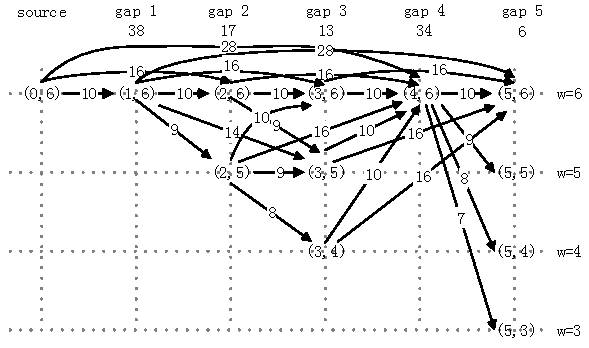
\includegraphics[width=0.7\linewidth]{sssp}
	\caption[sssp]{Here is a DAG for sequence with 6 integers represented using gap(differences between them). Optional bit widths range from 3 to 5, each gap is fitted in the tuple (\textit{position, available-bit-width}), if the available-bit-widths are more than one, they are placed in different rows, the number in the edge denotes the cost for this path, the fixed cost is set to 4.}
	\label{fig:sssp}
\end{figure}

The common foundation for the abovementioned methods is to recast the integer sequence $\mathcal{S} \left[ 0,n \right]$ to a particular DAG $\mathcal{G}$, each integer is represented by a vertex, plus a dummy vertex marking the end of the sequence, the graph $\mathcal{G}$ is complete, which means that for any $i$ and $j$ with $i < j \leqslant n$, there exists an edge connecting $v_{i}$ and $v_{j}$, denoted as $\left( v_{i}, v_{j} \right)$. In fact, the edge is an exact correspondence of a partition in the sequence $\mathcal{S}\left[i,j \right] $, the problem of fully partitioning $\mathcal{S}$ is converted to finding a path $\pi$ in $\mathcal{G}$, for instance, $\pi=\left( v_{0}, v_{i_{1}} \right) \left( v_{i_{1}}, v_{i_{2}} \right)\ldots\left( v_{i_{k-1}}, v_{n} \right)$ with $k$ edges corresponds to the partition $\mathcal{S}\left[0,i_{1}-1 \right]\mathcal{S}\left[i_{1},i_{2}-1 \right] \ldots\mathcal{S}\left[i_{k-1},n-1\right] $ of $k$ blocks. The weight of an edge in the graph is equal to the cost in bits consumed by the partition. Thus, the problem of optimally partitioning a sequence is reduced to the problem of Single-Source Shortest Path(SSSP) Labeling, as shown in Fig.~\ref{fig:sssp}. An intuitive way to solve this is to firstly set the cost of each vertex in $\mathcal{G}$ to $+\infty$, then an iteration starts from the left vertex to the rightmost, when it comes to a vertex $v_{j}$ with $0\leqslant j < n$, a subproblem of find the optimal path from $v_{j}$ to $v_{n}$ shows up, assuming the optimal path from $v_{0}$ to $v_{j}$ has been correctly computed. Each edge $\left( v_{j},v'\right)$ outgoing from $v_{j}$ will be assessed and cost of vertex $v'$ is updated if it becomes smaller. As can be seen, the time complexity of this algorithm is proportional to the number of edges in $\mathcal{G}$.

However, the $\mathcal{G}$ transformed from integer sequence $\mathcal{S}$ is complete with $\Theta\left( n^{2}\right)$ edges, especially some posting lists for popular terms will be quite large, finding their optimal partitions will be intolerable. Since dynamic programming is inefficient and greedy mechanism is too coarse, an elaborate approximation algorithm which reduces the time and space complexities to linear at the cost of finding slightly suboptimal solutions will be feasible.

\section{Optimizing Partitioning Strategy via Pruning DAG}\label{sec:optimization}

While PEF using Elias-Fano code gets an impressive compression performance, we are aiming at revitalizing encoders using binary packing with optimizations. Since Elias-Fano code compresses integer in its complete form which may leads to poor space efficiency, binary packing uses gapped integer instead will obtain better compression ratio, it is still an promising method with potential for faster compression speed.

\subsection{VSEncoding}

VSEncoding is similar to PFOR, however, it neither applies a fixed-sized block length nor appends a patch for outliers at the end of blocks. In order to maximize the compression while retaining simple and fast decompression, VSEncoding partitions each posting list into blocks of variable length, and binary packs the integers inside of each block with the number of bits, say \textit{b}, required to encode the largest one. Finally the the value of \textit{b} and the length of the block, \textit{k}, are encoded using distinct encoders $ \mathcal{M}_{1} $ and $ \mathcal{M}_{2} $. The basic form of each block can be seen as $ \{<k_{i},b_{i}>: data_{i}\}_{block_{i}} $, $ data_{i} $ is the $ k_{i} $ integers of $ block_{i} $ using $ b_{i} $ bits each.

Given a sequence $\mathcal{S}$ and a vector of partitions, the number of bits required to encode $\mathcal{S}$ can be computed in constant time, this quantity is calculated by summing up the costs of all the blocks, as the length of each block is variable, the problem of minimizing bits used relies on the problem of finding the optimal partitions. Let \textit{P} denote the vector of \textit{m} vertexes indicating the boundary of each block, with $ P\left[ 0 \right]  = 1 $, and $ P\left[ m \right]  = n $. The problem can be represented as follow:
\begin{equation*}
\min_{P\in\mathcal{S}}\sum_{i=0}^{m-1}c\left(P\left[i\right]-1,P\left[i+1\right]\right )
\end{equation*}
Where $c\left(P\left[i\right]-1,P\left[i+1\right]\right )=|\mathcal{M}_{1}\left( b_{i}\right) |+|\mathcal{M}_{2}\left( k_{i}\right) |+k_{i}b_{i}$, namely the cost to encode \textit{i}-th block.

VSEncoding adopts a dynamic programming algorithm to obtain the optimal partitions, each time a subproblem \textit{t} consists in encoding in the best way all the integers starting from 0 to \textit{t}, with a memo to look up when deciding whether to merge or split current partition. The whole procedure starts by setting $t = 0$ and goes down to $t = n$, which represents the solution to the original problem. In order to implement a faster algorithm, the block lengths are restrained to some small constants between 16 and 64, say \textit{h}, thus the time complexity drops from $ O\left(n^{2}\right) $ to $ O\left(n\log^{2}h\right) $.

To further improve decompression speed and keep the block representations word aligned, VSEncoding reorganizes the layout of blocks, first the description parts are stored together in their order (i.e., $,b_{0}k_{0},b_{1}k_{1}\dots,b_{m}k_{m}$), then the data parts are written separately into each group: first the values that have to be represented with 1 bit, then with 2 bits, and so on. The decompression procedure is done by binary-unpacking and permuting the data parts into the correct order according to description parts.

\subsection{Optimized Partitioning Strategy}

Next we describe our modification to VSEncoding that achieve significant improvements over its original version in \cite{silvestri2010vsencoding}. As mentioned before dynamic programming used in optimal partitioning costs too much time of index compression, to overcome this problem, we present a new partitioning scheme, which uses approximation algorithm in place of dynamic programming, thus reducing the time and space complexities to linear by finding a suboptimal partition. The partitioning problem can be reduced  to SSSP over a DAG $\mathcal{G}$ with $\Theta\left(n^{2}\right)$ edges, and its time complexity is proportional to the number of edges,
our aim is to design a pruning strategy removing edges of large costs while retaining edges which costs no more than $\left(1+\epsilon \right)$ times what the shortest paths do, for any given $\epsilon\in\left(0,1\right)$.

We use $c\left(v_{i},v_{j}\right)$ to denote the cost function of the edge $\left(v_{i},v_{j}\right)$, which is also the cost of a partition  $\mathcal{S}\left[i,j-1 \right]$, $U$ as the upper bound of cost by representing $\mathcal{S}$ as a single partition, and $F$ as the fixed cost of each partition(e.g. the descriptor). There is an obvious fact that, given any $0\leqslant i < j < k \leqslant n$, it is $ 0 < c\left(v_{i},v_{j}\right)\leqslant c\left(v_{i},v_{k}\right)\leqslant \ldots \leqslant c\left(v_{i},v_{n+1}\right)$.

By adopting a nontrivial pruning strategy a subgraph $\mathcal{G_{\varepsilon}}$ of the original $\mathcal{G}$ is produced, in which the shortest path and the suboptimal path which increases a little are preserved. Any edge $\left(v_{i},v_{j}\right)$ in $\mathcal{G_{\varepsilon}}$ follows at least one of the following conditions: 1) there exits a positive integer $k$ such that $c\left(v_{i},v_{j}\right) \leqslant F\left(1+\varepsilon\right)^{k} < c\left(v_{i},v_{j+1}\right)$\label{itm:property1}; 2)$j=n+1$. These edges of $\mathcal{G}_{\varepsilon}$ are called $ \varepsilon-maximal$ edges. As we have set the upper bound to $U$, there exists at most $\log_{1+\varepsilon}\frac{U}{F}$ possible values for $k$, thus for each vertex $\mathcal{G}_{\varepsilon}$ has at most $\log_{1+\varepsilon}\frac{U}{F}$ outgoing  $ \varepsilon-maximal$ edges. \cite{ferragina2011optimally} has proved that the shortest path distance on $\mathcal{G}_{\varepsilon}$, which is at most $\left(1+\varepsilon\right)$ times larger than the one in $\mathcal{G}$, can be computed in $O\left(n\log_{1+\varepsilon}\frac{U}{F}\right)$ time.

\begin{figure}
	\centering
	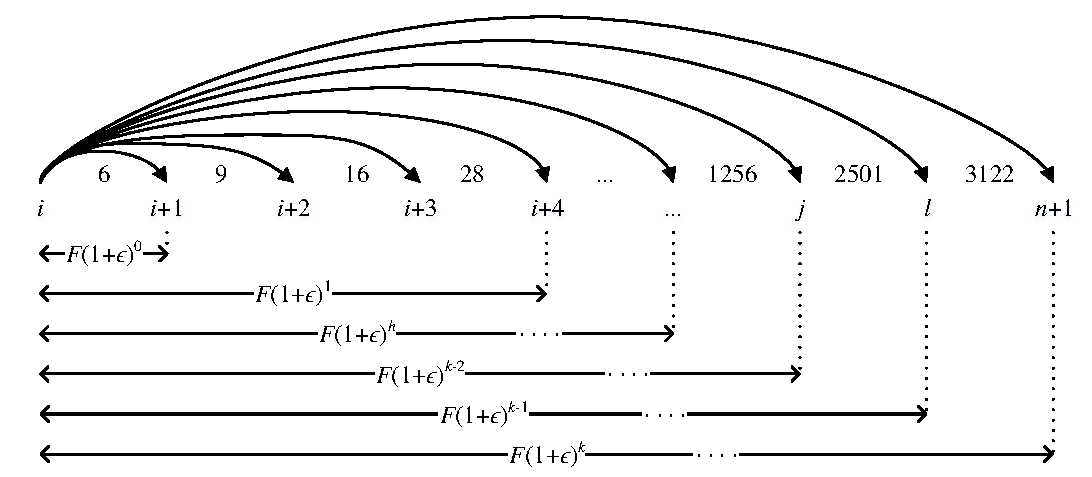
\includegraphics[width=0.7\linewidth]{sparsification}
	\caption[sparsification]{Curves represent outgoing edges from vertex $v_{i}$, the number under each curve is the cost of it, postulating the fixed cost is $F=4$. Lines below are cost classes with different $k$, for each class we can choose one edge as $\epsilon-maximal$ edge. This process is called sparsification.}
	\label{fig:sparsification}
\end{figure}

The above procedure is like the trimming scheme for the subset-sum problem\cite{cormen2009introduction}, which is to choose a representative for a compact range of its neighbor. In other words, we are sparsifying the complete graph $\mathcal{G}$ by quantizing its edge costs into classes of cost between $\left(1+\epsilon\right)^{i}$ and $\left(1+\epsilon\right)^{i+1}$, for each cost class of each node, only one $\epsilon-maximal$ edge is retained. If to prune $\mathcal{G}$ in a more coarse-grained but faster way, we can further remove edges which span too many vertex, intuitively, long edges are more vulnerable and sensitive to outliers, resulting in high cost and poor efficiency, thus are less likely to be enrolled in optimal partitioning. At the very beginning, we set the upper bound $U$ to be the cost of representing the whole sequence $\mathcal{S}$ as a single block, however this is an asymptotic upper bound which might never be reached, by refining $U$ to a more compact bound we can further lower the time complexity to linear without losing the approximation guarantees. Before giving our $U$ we first state the following proposition to be based on:

\begin{proposition}
	For any $0\leqslant i < j < k \leqslant n+1$, the weighting function satisfies $c\left(v_{i},v_{k}\right)+c\left(v_{k},v_{j}\right) \leqslant c\left(v_{i},v_{j}\right)+F+1$.
\end{proposition}

It is easy to prove as we split one edge into two shorter edges, the correspondent interval in $\mathcal{S}$ is also partitioned. The worst case is the split cuts out nothing but only adds cost of one descriptor. For any edge $\left(v_{i},v_{j}\right)$ in $\mathcal{G}_{\epsilon}$, we have $ c\left(v_{i},v_{j}\right) \leqslant \overline{U}$, if $c\left(v_{i},v_{j}\right)>\overline{U}$, then they are pruned and replaced by sub-edges in $\mathcal{G}_{\epsilon}$. These sub-edges can be found in a greedy way, in which the cost of each edge equals $\overline{U}$ (optimal ones are probably better), thus the number of edges cannot be larger than $\frac{c\left ( v_{i},v_{j} \right )-F}{\overline{U}-F}+1$. Postulating all the sub-edges are the worst cases which only add costs, the overall cost follows the inequality:
\begin{equation}
\sum_{i\leqslant k < l \leqslant j}c\left(v_{k},v_{l} \right ) \leqslant c\left(v_{i},v_{j} \right )+\left(\frac{c\left(v_{i},v_{j} \right )-F}{\overline{U}-F}+1\right)\left(F+1 \right )
\end{equation}
\noindent our ultimate goal is to keep the shortest path distance in $\mathcal{G}_{\epsilon}$ no more than $\left( 1+\epsilon\right)$ times the optimal one in $\mathcal{G}$, if $\left(v_{i},v_{j}\right)$ is one edge of the optimal path, we get the following inequality:
\begin{equation}
\sum_{i\leqslant k < l \leqslant j}c\left(v_{k},v_{l} \right ) \leqslant \left(1+\epsilon \right )\cdot c\left(v_{i},v_{j} \right )
\end{equation}
\noindent combining these two we get an inequality for $\overline{U}$:

\begin{equation}
\overline{U} \geqslant F+\frac{F+1}{\epsilon}
\end{equation}
\noindent One thing to be noted is that, even parameters $\epsilon$ and $F$ are predefined by user, there is an implicit criterion that for any edge $ \left(v_{i},v_{j} \right )$ the cost function must satisfy, since the correctness of pruning strategy relies on it: $\epsilon\cdot c\left(v_{i},v_{j} \right )-F-1>0$, which is not mentioned in \cite{ottaviano2014partitioned}. Different lower bound of $c\left(v_{i},v_{j} \right )$ determines the minimum of $\epsilon$, for instance, if $c\left(v_{i},v_{j} \right )\geqslant 2\left(F+1\right)$, then $\epsilon\in \left[ 0.5,1\right)$. Finally we can set our $\overline{U}$ to $F+\frac{F+1}{\epsilon} $, reducing the time complexity from $O\left( n\log_{1+\epsilon}\frac{U}{F}\right)$ to $O\left(n\log_{1+\epsilon}\frac{1}{\epsilon}\right)=O\left(n\right)$, more importantly, the approximation guarantee is preserved.

Even providing the edge cost can be computed in constant time, we cannot check every edge of the complete graph $\mathcal{G}$ to determine whether it is $\epsilon-maximal$ or not, since it would take $\Theta\left(n^{2}\right)$ time. To construct the pruned graph $\mathcal{G}_{\epsilon}$ on the fly we need to deploy a dynamic data structure that maintains a set of \textit{sliding windows} over $\mathcal{S}$ denoted by $\omega_{0},\omega_{1},\dots, \omega_{\log_{1+\epsilon}\frac{1}{\epsilon}}$, each of them represents a cost class of $F\left(1+\epsilon\right)^{k}$,  starting from the same vertex $v_{i}$ but covering a different range of $\mathcal{S}$. For each vertex $v_{i}$, each sliding window $\omega_{j}$ begins to expand its size from the starting position to the position where the cost is larger than $F\left(1+\epsilon\right)^{j}$ for the first time, thus we generate all the $\epsilon-maximal$ edges outgoing from $v_{i}$. By performing a scan on $\mathcal{S}$ for each sliding window, we get and evaluate all the $\epsilon-maximal$ edges on-the-fly. Thus, the algorithm returns the optimal partition in $O\left(n\log_{1+\epsilon}\frac{1}{\epsilon}\right)$ time.

\section{Experiments}\label{sec:experiments}

\subsection{Experimental Setup}

In our experiments, we use the posting lists extracted from the TREC GOV2 collection, which consists of 25.2 million web pages and about 32.8 million terms in the vocabulary crawled from the gov Internet domain. The uncompressed size of these web pages is 426GB. Also, all the terms have the Porter stemmer applied, and stopwords have been removed, docids are assigned in two ways: according to the lexicographic order of their URLs or to the order that they appear in the collection, thus we can see how docid reordering influence indexing performance. Then the docids and term frequencies are extracted from the collection in a non-interleaved way and applied with compression methods separately. To highlight the improvements between the original methods and our optimizations, the compression methods used in experiments are AFOR, VSEncoding via Dynamic Programming (VSE-DP) and VSEncoding via Optimal Partitioning (VSE-OP), we do not compare other methods like the Simple Family or PFOR in our benchmark as they have been throughly studied in the literature\cite{catena2014inverted,lemire2015decoding,ottaviano2015optimal,yan2009inverted}.

All the implementations are carried out on an Intel(r) Xeon(r) E5620 processor running at 2.40 GHz with 128GB of RAM and 12,288KB of cache. The default physical block size is 16KB, algorithms are implemented using C++ and compiled with GCC 4.8.1 with –O3 optimizations. In all our runs, the whole inverted index is completely loaded into main memory, in order to warm up the execution environment, each query set is run 4 times for each experiment, and the response times only measured for the last run. Our implementations are available at \url{https://github.com/Sparklexs/myVS}.

\subsection{Indexing Performance}

The performance of indexing is based on the index size and compression speed. Before comparing the spaces obtained by different methods, we first set the parameters needed by AFOR, as mentioned before, to keep byte-aligned, we set the frame length to be (8, 16, 32), these configurations give the best balance between performance and compression ratio. Offering additional frame lengths will slightly increase the compression ratio, at the cost of linearly decreasing the compression speed.

\begin{table}
	\caption[index size]{Total Size in GB, and corresponding average bits per integer(bpi) for docid and frequency, compressed by different methods on GOV2}
	\begin{center}
		\renewcommand{\arraystretch}{1.4}
		\setlength\tabcolsep{6pt}
		\begin{tabular}{c*{2}{*{2}{>{\columncolor[gray]{.9}}r}rr}}
			\toprule
			\multirow{2}*{methods}& \multicolumn{4}{c}{original} & \multicolumn{4}{c}{reordered} \\ \cmidrule(lr){2-5} \cmidrule(lr){6-9}
			& \multicolumn{1}{c}{docid} & \multicolumn{1}{c}{bpi} & \multicolumn{1}{c}{freq} & \multicolumn{1}{c}{bpi} & \multicolumn{1}{c}{docid} & \multicolumn{1}{c}{bpi} & \multicolumn{1}{c}{freq} & \multicolumn{1}{c}{bpi} \\ 
			\midrule

			AFOR & 16.30 & 30.17 & 8.10 & 14.95 & 9.78 & 18.05 & 6.39 & 11.81 \\
			VSE-DP & 4.13 & 7.64 & 2.08 & 3.84 & 1.97 & 3.65 & 1.89 & 3.50 \\
			VSE-OP & 4.22 & 7.80 & 2.25 & 4.17 & 2.04 & 3.76 & 2.04 & 3.77 \\
			\bottomrule
			\label{tab:index size}
		\end{tabular}
	\end{center}
\end{table}

Table~\ref{tab:index size} shows the index space, it is divided into two classes, the original and the reordered, the former denotes docids are assigned in the order they appear and the latter denotes docids are assigned in the lexicographic order of their URLs. The overall size and bits per integer of docid and frequency are shown separately. To facilitate reading, we fill docid-related cells with gray, so are the other tables below. We can observe that VSE-OP gets slightly worse result than its initial version, since we are focusing on accelerating compression speed, the partitioning scheme we adopt in VSE-OP is suboptimal, but it is still competitive compared with the optimal one. We can also observe VSEncoding achieves far more better compression ratio than AFOR, no matter for docid or frequency, the size of AFOR is nearly 4 times larger than VSEncoding, which demonstrates that a partitioning strategy, which offers more optional frame lengths, can more effectively utilize the distribution of integers to compress the sequence. Also note that docid after reordering is half the size it is ordered by the sequence of appearance, while frequency stays less sensitive to reordering, this can be explained by the fact that docid is stored in ascending order and reordering by URL further narrows the gaps between consecutive docids, however the frequency is aligned with docid and stored in an unordered way, thus reordering does not make too much difference. Also the docids are quite sparse while the frequencies are fairly concentrated, rendering the docid's compression ratio twice larger than the frequency's. 

\begin{table}
	\caption[compression speed]{Total time elapsed in seconds and performance in million integers per second(mis) when compressing docid and frequency}
	\begin{center}
		\renewcommand{\arraystretch}{1.4}
		\setlength\tabcolsep{6pt}
		\begin{tabular}{c*{2}{*{2}{>{\columncolor[gray]{.9}}r}rr}}
			\toprule
			\multirow{2}*{methods}& \multicolumn{4}{c}{original} & \multicolumn{4}{c}{reordered} \\ \cmidrule(lr){2-5} \cmidrule(lr){6-9}
			& \multicolumn{1}{c}{docid} & \multicolumn{1}{c}{mis} & \multicolumn{1}{c}{freq} & \multicolumn{1}{c}{mis} & \multicolumn{1}{c}{docid} & \multicolumn{1}{c}{mis} & \multicolumn{1}{c}{freq} & \multicolumn{1}{c}{mis} \\ 
			\midrule
			AFOR & 78.98 & 58.95 & 72.56 & 64.17 & 75.43 & 61.72 & 66.92 & 69.58 \\
			VSE-DP & 8303.96 & 0.56 & 8005.42 & 0.58 & 7849.07 & 0.59 & 7966.30 & 0.58 \\
			VSE-OP & 5982.24 & 0.78 & 5819.72 & 0.80 & 5601.14 & 0.83 & 5648.14 & 0.82 \\
			\bottomrule
			\label{tab:compression speed}
		\end{tabular}
	\end{center}
\end{table} 
                            
Table~\ref{tab:compression speed} shows the compression speed of different methods when constructing index for docid and frequency. Combining with the index size shown in Table~\ref{tab:index size}, we can find that there is a clear trade-off between compression efficiency and effectiveness, while index compressed by AFOR is quadruple the size of the ones compressed by VSEncoding, however, its compression speed is two orders of magnitude faster than VSEncoding. Due to a lack of attention, the construction time of experimented methods are rarely mentioned in the literature, we cannot find their performances on other platforms to compare. In our experiment, the optimized method outperforms its original version, the average time saved constitutes nearly 20\% of the time cost by the original. We can notice that the performance gap between docid and frequency is not very apparent, for that they contain the same number of integers. Also, the compression methods traverse the lists in a fixed way, which is irrelevant to the symbols the lists may contain. The only difference exists is that docid is sparser and larger than frequency, thus leading to the result that compressing docid is a little more time-consuming than compressing frequency. One exception is that VSE-OP partitions a list under the influence of the predefined parameter $\epsilon$ and the upper bound of representing the list in a single block, we can observe that compression speed between docid and frequency using VSE-OP is quite different. Another thing to be noted is that compressing reordered lists cost less time than the original lists both for docid and frequency.

Table~\ref{tab:loops count} further details the performance of different methods. As is shown, Table~\ref{tab:loops count} lists the number of partitioning schemes evaluated when traversing the integer sequences, comparing these different encoders, we can see that the partitioning step is crucial for compression speed. The optimized method sharply reduces the calculation needed to partition a posting list. By pruning edges with large cost, more than half of the calculation is saved by VSE-OP. We can also note that all methods maintain the same calculation in the four columns except VSE-OP, it is easy to explain by the fact that time complexities of the first two methods are only relevant to the length of input sequences, while VSE-OP is relevant to both the length and the upper bound of the sequences. Calculation of frequency for VSE-OP stays the same after reordering because the changed integer distribution makes no difference to the upper bound of the sequence. However calculation for docid is slightly reduced as upper bound of the sequence is narrowed.

\begin{table}
	\caption[loops count]{Number of evaluated partitions by different methods}
	\begin{center}
		\renewcommand{\arraystretch}{1.4}
		\setlength\tabcolsep{6pt}
		\begin{tabular}{c*{2}{>{\columncolor[gray]{.9}}rr}}
			\toprule
			\multirow{2}*{methods}& \multicolumn{2}{c}{original} & \multicolumn{2}{c}{reordered} \\ \cmidrule(lr){2-3} \cmidrule(lr){4-5}
			& \multicolumn{1}{c}{docid} & \multicolumn{1}{c}{freq} & \multicolumn{1}{c}{docid} & \multicolumn{1}{c}{freq} \\ 
			\midrule
			AFOR & 718,920,570 & 718,920,570 & 718,920,570 & 718,920,570 \\
			VSE-DP & 293,805,525,502 & 293,805,525,502 & 293,805,525,502 & 293,805,525,502 \\
			VSE-OP & 128,325,159,726 & 126,661,641,588 & 111,438,988,684 & 126,661,641,588 \\
			\bottomrule
			\label{tab:loops count}
		\end{tabular}
	\end{center}
\end{table}

\subsection{Decompression Performance}

In this subsection, we are going to discuss the decompression performance of different methods, before reporting our results on the decompression speed, we first display the distribution of partition lengths, which can help us in understanding the differences among these partitioning schemes, and the correlation between clusters in a collection and partitions produced on it by variant methods.

As is discussed before, AFOR and VSE-DP use a partitioning strategy with fixed-sized lengths (8, 16, 32 for AFOR, and 1, 2, 4, 6, 8, 16, 32, 64 for VSE-DP), while VSE-OP uses a more flexible partitioning strategy, its partition lengths are determined by a series of sliding windows when traversing the sequence. To show the distribution clearly, we display the first two methods in histograms and VSE-OP in scatter plots as shown in Fig.~\ref{fig:bcHistogram} and Fig.~\ref{fig:bcScatter}.

\begin{figure}
	\centering
	\subfigure[docid]{
		\label{fig:subfig:a}
		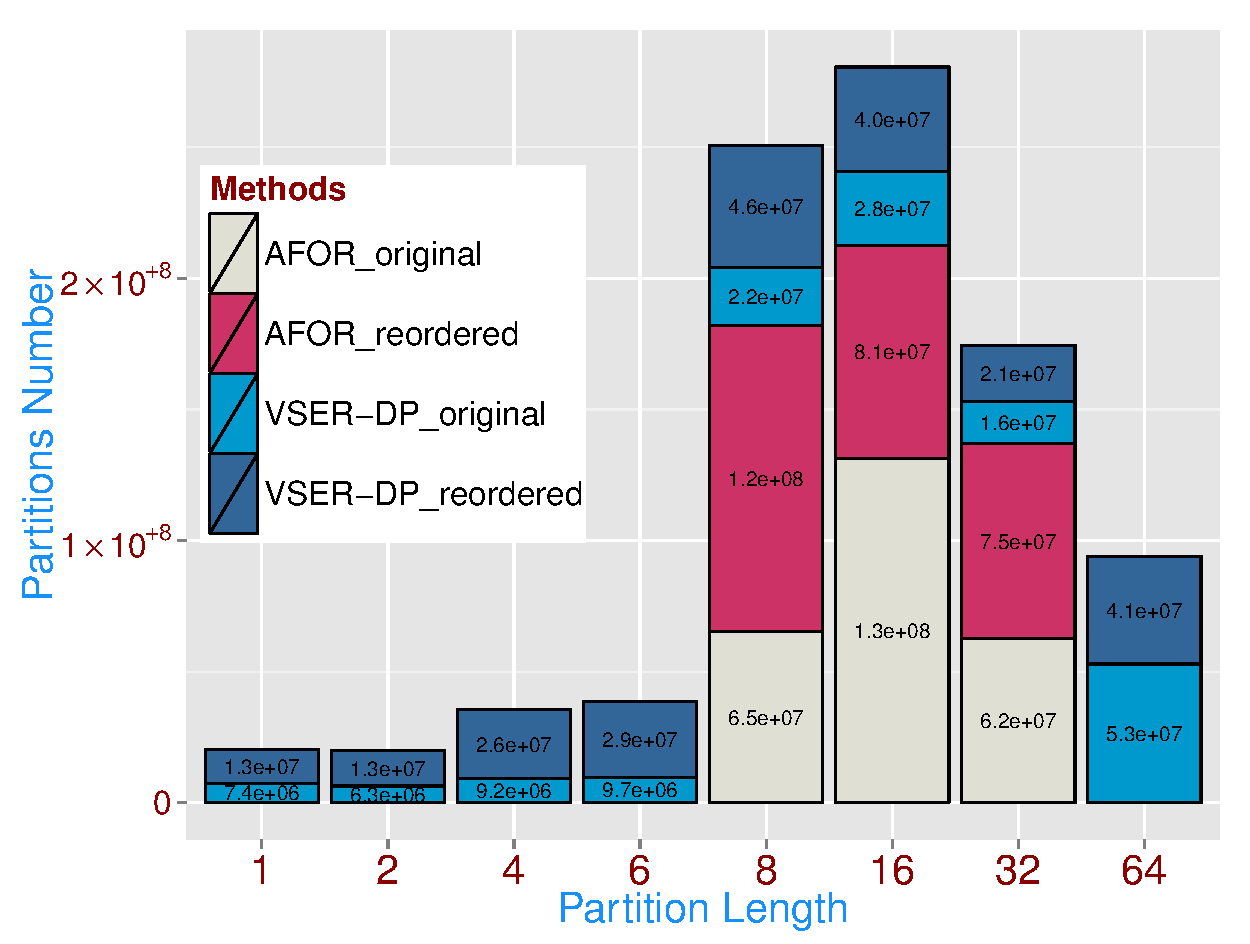
\includegraphics[width=0.47\linewidth]{bcDocidNoKAFOR}
	}
	\subfigure[frequency]{
		\label{fig:subfig:b}
		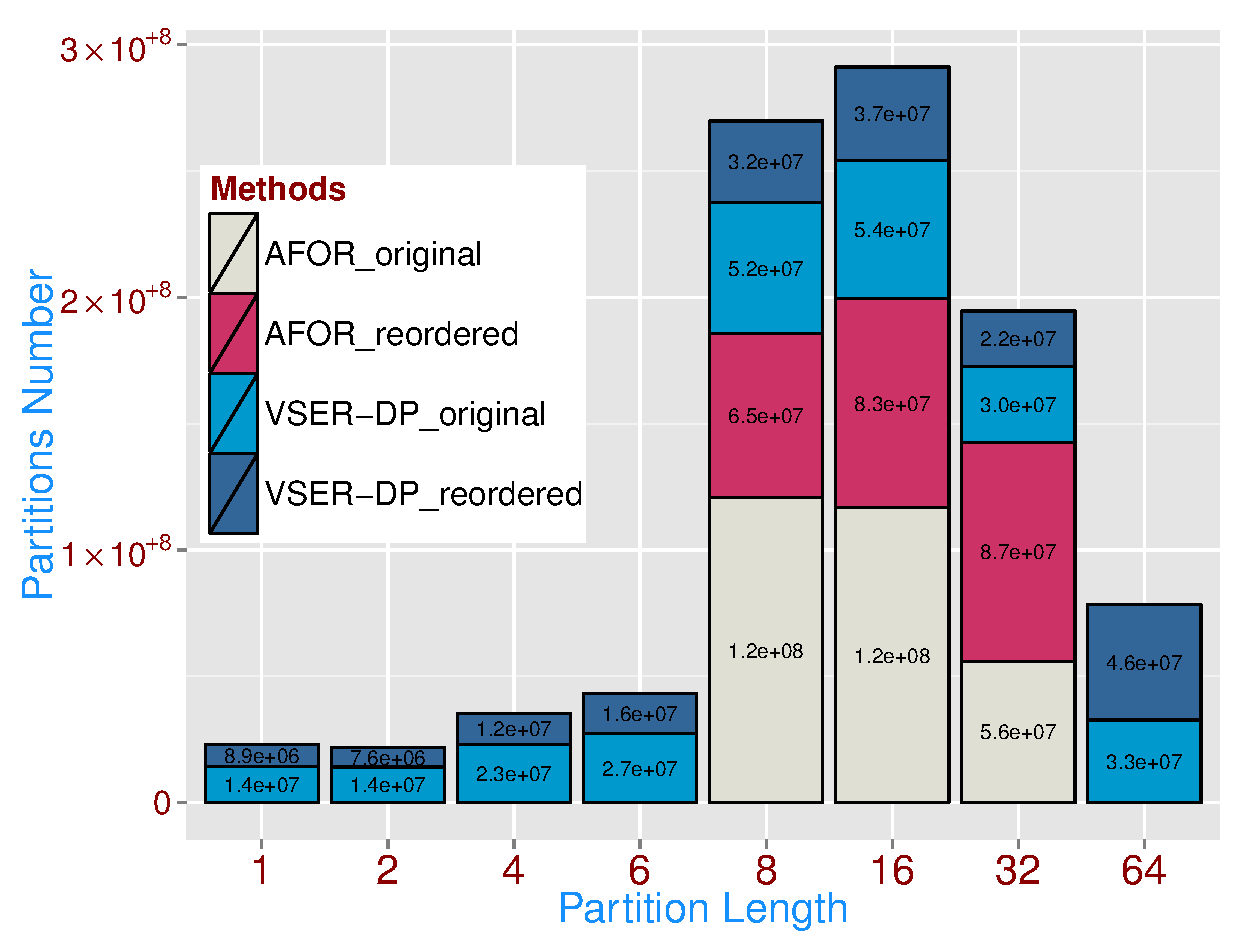
\includegraphics[width=0.47\linewidth]{bcFreqNoKAFOR}
	}
	\caption[distribution of partition lengths 1]{distribution of partition lengths produced by AFOR and VSE-DP}
	\label{fig:bcHistogram}
\end{figure}

There is one important proposition we need to declare: there exists a compromise among partition length, compression ratio, compression and decompression speed. All the codewords that fall into one partition share the same bit width, thus the smaller the partition length is, the less bits will be wasted, however, smaller partition lengths also produce more fragmentations in one sequence, resulting in more CPU cycles and disk I/O needed to write and read these partitions. Vice versa, larger partition lengths are easier to access but less space-friendly. In Fig.~\ref{fig:bcHistogram}, each bar indicates number of specified lengths used by one or more methods in pairs, each two adjacent blocks in one bar indicate the different number before and after reordering for one method, more exactly, the pale color represents the original and the dark color represents the reordered.

Fig.~\ref{fig:subfig:a} shows that after reordering these two methods produce more blocks with small lengths than before, so the compressed size contracts sharply. However, these methods produce more large lengths on frequency as shown in Fig.~\ref{fig:subfig:b}, resulting an inferior compression ratio than that on docid. When it comes to decompression speed (which will be listed below in Table~\ref{tab:decompression speed}), larger partitions imply faster access speed for a list of integers. From Fig.~\ref{fig:bcHistogram}, we can find that AFOR has larger partition length than VSE-DP, so the disk I/O for it decreases orderly, however this only includes the disk transfer time, their time complexities on calculation do not change. Overall, these methods do not have a large variation in terms of partition lengths, which shows that they are able to adapt to the skewness of a dataset.

\begin{figure}
	\centering
	\subfigure[docid]{
		\label{fig:subfig:c}
		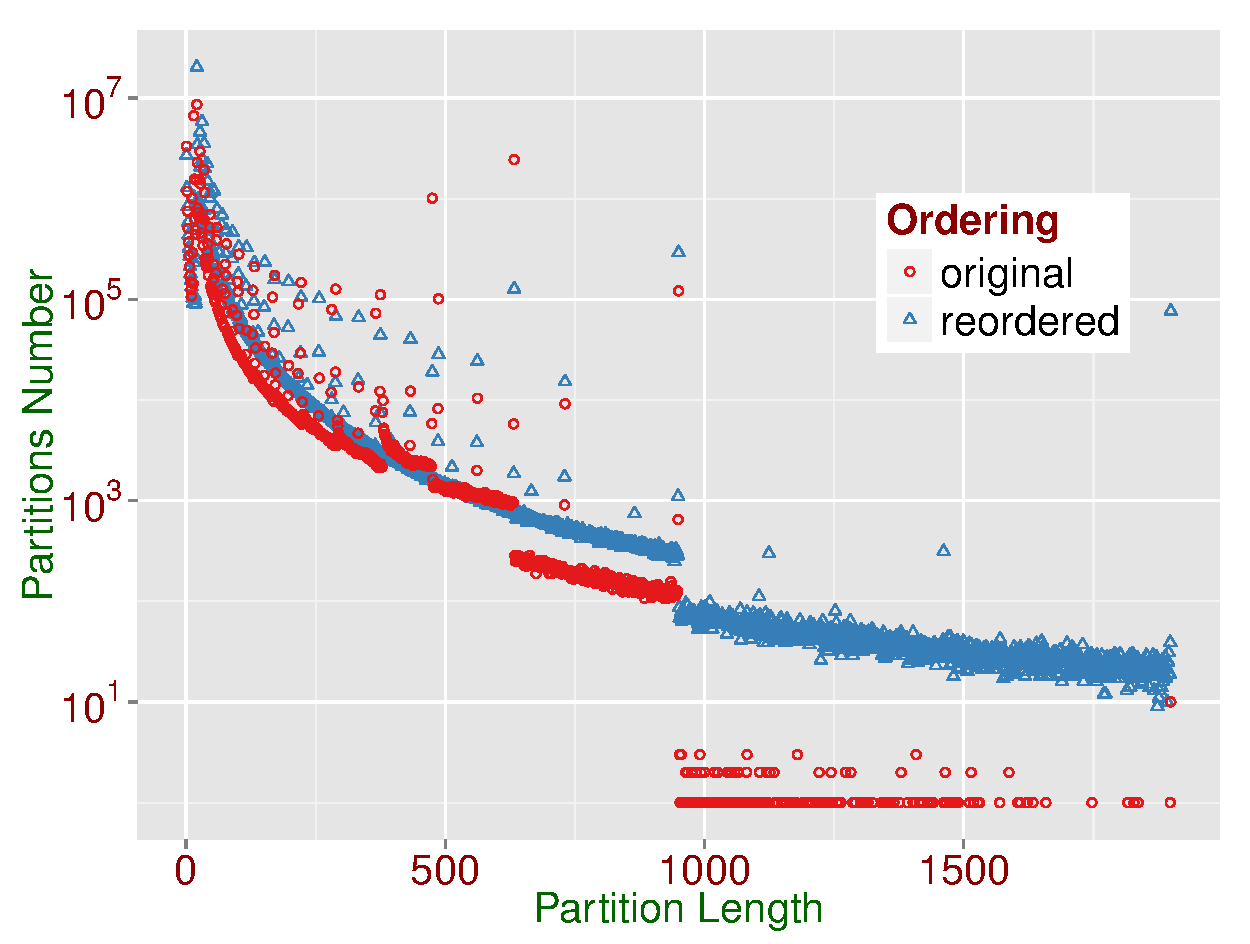
\includegraphics[width=0.47\linewidth]{OPDocid}
	}
	\subfigure[frequency]{
		\label{fig:subfig:d}
		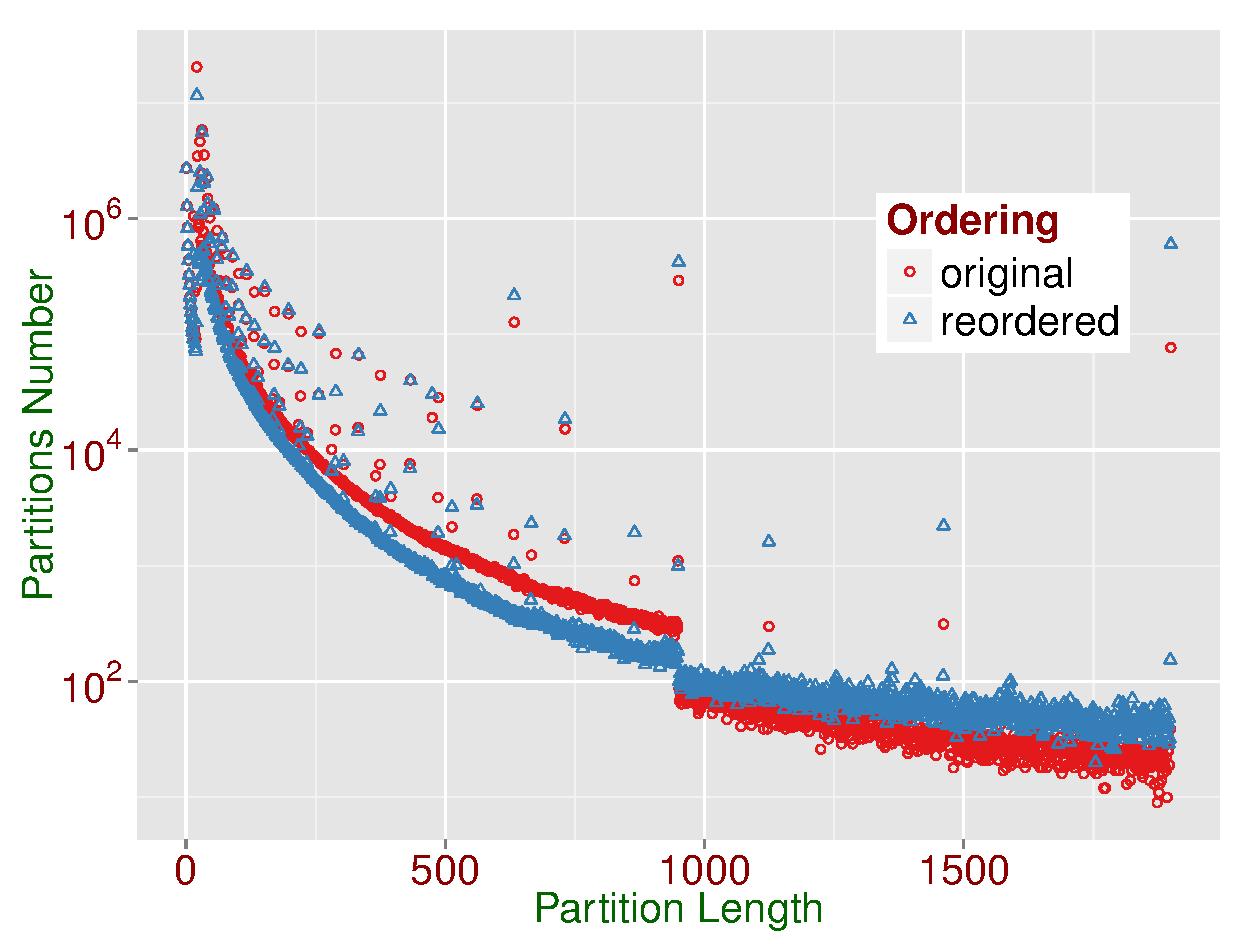
\includegraphics[width=0.47\linewidth]{OPFreq}
	}
	\caption[distribution of partition lengths 2]{distribution of partition lengths produced by VSE-OP}
	\label{fig:bcScatter}
\end{figure}

Things go quite different for VSE-OP: as shown in Fig.~\ref{fig:bcScatter}, the partition lengths vary from 0 to larger than 1500 rather than being confined to a small range. In order to improve the interpretability of the result, we apply \textit{log transformation} to the original graph. As for the docid on the left hand, we can observe that partitions shorter than 500 compose the main proportion of the whole distribution, at the point of 1000, there exists a sharp segmentation, specially for the docid without reordering, number of such partitions drops to 1. However, reordering increases the number by almost one order of magnitude. With much more long partition allocated, VSE-OP still keeps its compression ratio close to VSE-DP, this  illustrates its superiority on choosing partitions while avoiding wasting space caused by outliers. Also, different from Fig.~\ref{fig:bcHistogram}, with quantity of longer partitions growing, size of VSE-OP after reordering decreases to half of the original as shown in Table~\ref{tab:index size}, which again confirms that long partitions chosen by VSE-OP do not add load on space occupancy. Fig.~\ref{fig:subfig:d} for frequency shows similar result with that for docid, the only difference is that reordering does not affect the distribution as acutely as that in Fig.~\ref{fig:subfig:c}, this can be explained by the fact that reordering has no effect on the value range of frequency sequences.

\begin{table}
	\caption[decompression speed]{Total time elapsed in seconds and performance in million integers per second(mis) when decompressing docid and frequency}
	\begin{center}
		\renewcommand{\arraystretch}{1.4}
		\setlength\tabcolsep{6pt}
		\begin{tabular}{c*{2}{*{2}{>{\columncolor[gray]{.9}}r}rr}}
			\toprule
			\multirow{2}*{methods}& \multicolumn{4}{c}{original} & \multicolumn{4}{c}{reordered} \\ \cmidrule(lr){2-5} \cmidrule(lr){6-9}
			& \multicolumn{1}{c}{docid} & \multicolumn{1}{c}{mis} & \multicolumn{1}{c}{freq} & \multicolumn{1}{c}{mis} & \multicolumn{1}{c}{docid} & \multicolumn{1}{c}{mis} & \multicolumn{1}{c}{freq} & \multicolumn{1}{c}{mis} \\ 
			\midrule
			AFOR & 36.53 & 127.04 & 31.24 & 148.55 & 33.01 & 140.56 & 28.77 & 161.36 \\
			VSE-DP & 69.09 & 67.17 & 71.97 & 64.48 & 52.98 & 87.60 & 70.11 & 66.19 \\
			VSE-OP & 48.24 & 96.20 & 49.81 & 93.16 & 40.15 & 115.58 & 48.56 & 95.56 \\
			\bottomrule
			\label{tab:decompression speed}
		\end{tabular}
	\end{center}
\end{table}

Table~\ref{tab:decompression speed} reports the results on  decompression speed, again our optimized method outperforms its original version. The decompression speed are much faster than the compression speed, however, with more partitions included, VSEncoding will encounter more skips when decompressing, which slows down its speed; on the other hand, long partitions also enable decompressing more integers in bulk. In a nutshell, the speed achieved by VSEncoding, specially by VSE-OP, is still competitive with AFOR, taking the compression ratio into account. Restrained by the configuration of our platform, the results in our experiment are quite different from that in \cite{silvestri2010vsencoding}, where VSE-DP is said to reach a speed of $450\pm20$ mis.

\section{Conclusion and Future Work}\label{sec:conclusion}

In this paper we introduced and motivated the study of shortening compression time of inverted index via optimizing partitioning strategies. We first summarized a series of compression techniques which fall into the same category by treating the partitioning problem as SSSP over a DAG. Then we presented our optimization on VSEncoding with a better space-time trade-off, namely to enhance its partitioning procedure with more flexibility and faster speed, while keeping its compression ratio and decompression speed competitive. At last, an extensive experimental analysis was given, which showed that our optimization significantly improve the compression speed as well as the decompression speed, with a little loss at in space efficiency.

There are still many open problems and opportunities for future research, since our solution only focus on optimizing VSEncoding, further experiments will investigate the consequence of optimizing other compression techniques and design a compression that offers better space-time trade-offs. An interesting problem would be using SIMD instructions to further accelerate the compression and decompression speed, also it would be promising to decrease the time complexity of the approximation algorithm adopted to compute optimal partitions.

\bibliographystyle{splncs03}
\bibliography{reference,reference_intersection}

\end{document}
